\documentclass{article}
\usepackage{amsmath}
\title{Diskretka 3}
\author{Hynek Kydlíček}
\usepackage{graphicx}
\usepackage{ amssymb }
\graphicspath{{./}}
\begin{document}
\section{Úkol 1}
Nespočetně mnoho neizomorfních uspořádání.\\
Uspořádání zadefinujeme pro každé $n >= 2$ následovně.
Nejprve seřadíme všechna čísla $x \in N$, která jsou dělitelná $i=2$ neostrou nerovností.
Poté zbylá čísla, která jsou dělitelná $i=3$. Takto řadíme až do doby, dokud $i \le n$.
Nakonec seřadíme všechna zbylá čísla neostrou nerovností.
Každé dvě takové uspořádání jsou neizomorfní.
Rozdělíme si uspořádání na množiny $M_2$ \dots $M_N$, podle toho, jak jsme uspořádání kontruovali.V množině $M_2$ jsou čísla dělitelná 2, v množině $M_3$ jsou zbylá čísla dělitelná 3, až v $M_N$ jsou zbylá čísla. Každé dvě uspořádání $R_1, R_2$ se jistě liší v počtu takových množin.
Určitě tedy bude existovat množina $M_{N-1}$, která bude bude v jendom uspořádání a v druhém ne.
Kvůli této množině nejsme schopni najít bijekci, protože množina je nekonečně velká.
Mezi množinami $R_1_{M_i}$ a $R_2_{M_i}$ bijekci najdeme, ale poté nám zbyde $R_1_{M_N}$ a $R_2_{M_N-1}, R_2_{M_N}$, pro tyto množiny bijekci nenajdeme.

\section{Úkol 2}
Dokážeme pro obecnou funkci $f X -> Y$, kde X,Y jsou neprázdné\\
Většina důkazů využívá, že $(\forall x \in X) (!\exists y \in Y)$, explicitně jsem to zmínil pouze při reflexivitě, ale u susbtitucí to používám také.
\subsection{Reflexivita}
$xRx \iff f(x) = f(x)$, z definice funkce $(\forall x \in X)(!\exists y \in Y)$
a tedy $xRx$ platí pro každou funkci.
\subsection{Symetrie}
$(xRy \iff f(x) = f(y)) \rightarrow (yRx \iff f(y) = f(x))$,
pokud platí $f(x) = f(y)$, substitujeme $f(x)$ za $f(y)$ a naopak v předpokladu a dostávame, $f(y) = f(x)$, tedy $yRx$
\subsection{Tranzitivita}
Ukážeme, že když platí $xRy \wedge yRz \rightarrow xRz$.
Tedy platí $f(x) = f(y) \wedge f(y) = f(z)$, z definice funkce má $f(x)$ stejnou hodnotu jako $f(y)$, proto můžeme psát, že
$f(x) = f(z)$, tedy $xRz$.
\\
Jinak.
$(xRy \iff f(x) = f(y)) \wedge (yRz \iff f(y) = f(z)) \rightarrow (xRz \iff f(x) = f(z))$, substitucí druhého předpokladu do prvního dostáváme, že $f(x) = f(z)$, a tedy $xRz$ platí.
\pagebreak
\section{Úkol 3}
Výsledné relace nemusí být ani uspořádání natož lineární.\\
\textbf{Protipříklad:}\\
Množina, kterou budeme uspořádávat je $\{1,2,3,4\}$. Definujme na ni následující uspořádání(vztahy plynoucí z tranzitivity jsem nekreslil, aby byl obrázek přehledný,ale pro úplnost u modrého uspořádání ještě platí (1,3),(1,4) a (2,4))\\
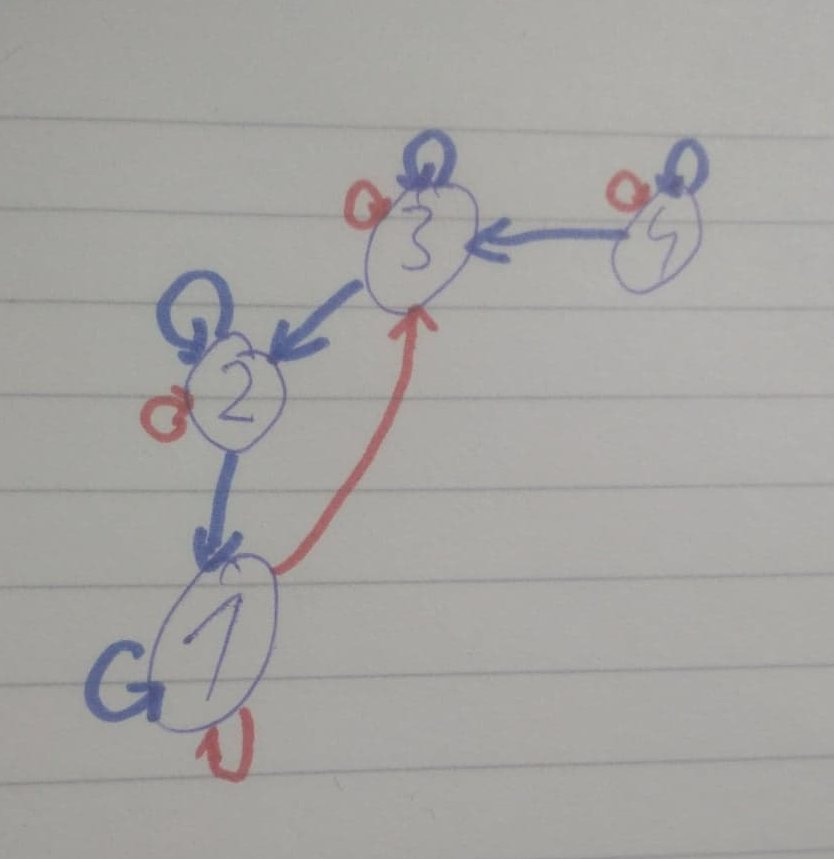
\includegraphics[scale=0.2]{3.jpg}\\
\textbf{Červené šipky jsou částečné uspořádání a modré lineární.}\\
Předpokládejme, že vzniklá relace je uspořádání. Poté platí. $2 \preceq 3, 1 \preceq 2, 3 \preceq 1$. Protože ale $1 \preceq 2$ a $2 \preceq 3$ pak $1 \preceq 3$. Nastal spor, protože relace má být uspořádání, ale relace není antisymetrická.

\section{Úkol 4}
Množinu $\{1,2...100\}^2$ si označme M.\\
notace $[x]$ znamená $\{1\dots{x}\}$
\subsection{Nejdělší řetězec je délky 199}
Vypadá takto: $\{(a,b) \mid (a,b) \in M \wedge  a + 1 = b\}\ \cup$ $\{(a,b) \mid (a,b) \in M \wedge  a = b\}$. Prvků v první množině je určitě $99$. Prvků v druhé je $100$. Množinu si můžeme představit tak, že přidáváme $+ 1$ cik-cak k $a,b$. Takže $(1,1),(1,2),(2,2),(2,3)\dots(100,100)$. O řetězec se jedná, neboť každé dva prvky spolu určitě budou porovnatelné(další prvek vytvoříme přidáním 1, tedy všechny prvky vytvořené předtím budou určitě menší).
Ukážeme, že řetězec delší než 199 nemůže existovat. Množinu M rozdělíme na antiřetězce, takže
\begin{equation}
    \begin{split}
    \{\{(i, k+1-i)\ \mid i \in [k] \} \mid k  \in [99]\} &\cup \{\{(100-k+i, 101-i)\} \mid i \in [k] \} \mid k  \in [99] \}\\
        &\cup \{\{k,101-k\} | k \in [100]\}
    \end{split}
\end{equation}
O antiřetězce se určitě jedná. Z kontrukce vidíme, že "sousední prvky" se liší o (a-1, b+1), tedy pro každé dva prvky $(a, b), (c, d)$ v antiřetězci platí, že $ (a < c \wedge d < b) \vee (a > c \wedge d > b)$. Zároveň je z kontrukce jasné, že antiřetězců je 199 a pokrývají celou množinu.
Pro názornější představu, jak vybrat antiřetězce, jsem udělal nákres \ref{fig:ret}.
\begin{figure}[htpb]
    \centering
    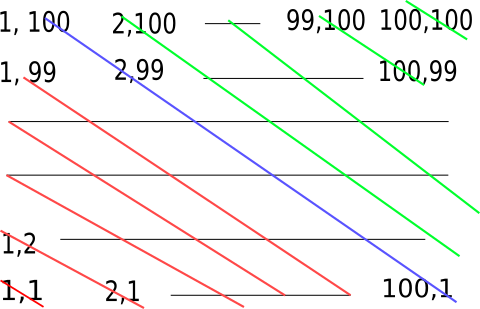
\includegraphics[width=0.4\linewidth]{4.png}
    \caption{množina 1 (červená), množina 2 (zelená), množina 3 (modrá)}%
    \label{fig:ret}
\end{figure}
Množinu jsme tak celou rozdělili na 199 antiřetězců, a jelikož každý antiřetězce může obsahovat maximálně jeden prvek z nejdelšího řetězec je tím důkaz hotov.

\subsection{Nejdělší antiřetězce je délky 100}
Vypadá takto: $\{(i,101-i) \mid i \in [100]\}$. Prvků v množině je určitě 100. O antiřetězec se jedná, neboť pro každé dva prvky (a,b) a (c,d) platí že $a < c \rightarrow b > d$ a $a > c \rightarrow b < d$ a zárověn nemůže nastat, že $a=c$.
Ukážeme, že antiřetězec delší než 100 nemůže existovat. Množinu M rozdělíme na řetězce tak, že $ \{\{(i,j) \mid j \in [100]\} \mid i \in [100]\}$. Řetězce tedy budou vypadat následovně: $\{(1,1),(1,2),\dots (1,100)\},\{(2,1),(2,2),\dots (2,100)\},\dots,\{(100,1),(100,2),\dots (100,100)\}$.Množinu jsme tak celou rozdělili na 100 řetězců, a jelikož každý řetězce může obsahovat maximálně jeden prvek z nejdelšího antiřetězce, je tím důkaz hotov.

\end{document}
